% the main points of this introduction are 
% outline the complexity of biological systems for physicists
% 	> even though our theoretical models should preidct everything on the energy and length scales of biology we can't because of their heterogeneity.
%   > Give examples of the heterogenaity 
% Give some points on the history of molecular biophysics  
%   >  Hodgkin-Huxley Models
%   > Gramicidin 
% Point out how Cystic Fibrosis is an expression of this progression, going from genotype to phenotype using an ion channel to teach us biophysics. 
% conclusion.
\chapter{An Introduction to Physical Biology}
\pagenumbering{arabic}
\setcounter{page}{1}
\label{chap:introduction}
\chapquote{Whatever complexity means, most people agree that biological systems have it.} {-Frauenfelder and Wolynes \cite{frauenfelder1994}}
\vspace
\section{Thesis and Chapter Summary}

This thesis seeks to apply a philosophy of molecular biophysics to demonstrate its capability to investigate pressing problems in biology and medicine. In particular, we will use molecular dynamics (MD) to look at how a specific gene misfunctions when expressed as a protein, the Cystic Fibrosis Transmembrane Conductance Regulator (CFTR), to cause a disease (CF). These MD techniques will allow us to formulate a model of CFTR's misfunction which we hope will direct research efforts and allow more patients suffering from CF access life saving medication. 

In this first short chapter we will quickly build a philosophy of how to look at biology through the lens of a physicist. We will outline what the goal of a physicist is, to create abstract formalisms which can be used to model the natural world. We will then observe what makes the construction of such formalisms so difficult in biology. We will walk through how a specific protein ion channels have historically served as laboratories to help understand aspects of more complex biological systems, such as whole cells or organisms. 

Chapter \ref{chap:methods} will describe the chemical and numerical simulation techniques we have used to study the CFTR protein system in detail, while chapter \ref{chap:cftr} gives an overview of the CFTR system itself, and also a set of \textit {in vitro} assays which compliment our computational modelling.  Chapters \ref{chap:i37r}, \ref{chap:r352q}, \ref{chap:s945l} and \ref{chap:opening} demonstrate the details of how a diverse application of the simulation techniques in chapter \ref{chap:methods} can be used to discover the unique modes of misfunction in CFTR. In combination with \textit {in vitro} cellular techniques, these simulation results prove that these mutations can be rescued by existing drug regimens. Finally, chapter \ref{chap:conclusion} ties together these results to argue for a physical model which elucidates the mechanism of action for cystic fibrosis drugs. Armed with this model we will work through the available literature and identify some priorities for future studies using molecular modelling for cystic fibrosis research.

We hope this small example can demonstrate the utility of physics expertise for the field of molecular medicine. We anticipate that such methods will only grow in power with improvements in computational and experimental techniques.

\section{What is Physics?}
\label{WIP}
When I was in high school I always described physics as ``the study of how things move". Although intuitive, this description does not shed light on the philosophy of doing physics which make it such a powerful tool for understanding the natural world. To create a predictive physical, theory one must first carefully define a naturally motivated formalism. Then, using mathematics, the implications of this formalism are built up to make predictions about measurable phenomena. Should the predictions from the formalism agree with experimental results, it validates the physical theory. This is what makes physics feel like the most ``fundamental" of the natural sciences.\footnote{The natural sciences include chemistry, biology, physics.  Mathematics and logic are forms of the formal sciences, which we rely on heavily as natural scientists. }

These formalisms use an array of mathematical structures. Examples include:
\begin{itemize}
\item The gas of hard spheres, which we use to derive the Boltzmann's kinetic theory of gasses.  
\begin{equation}
	\label{hard_spheres}
	\frac{\partial f_1}{\partial t} + \frac{\bold{F}}{m}\cdot\nabla_\bold{r} + \bold{v} \cdot \nabla_\bold{r} f_1 =  \int \int (f'_1f'_2 - f_1 f_2) \tilde \kappa d \hat \kappa d \bold{v}_2
\end{equation}

\item The interacting electric and magnetic vector fields in Maxwell's laws of electromagnetism.
\begin{equation}
	\begin{aligned}
	%\nabla \dot \mathbf{E} = \frac{\rho}{\epsilon_0}
		\nabla \cdot  \mathbf{E} &= \frac{\rho}{\epsilon_0} \qquad & \nabla \cdot  \mathbf{B} &= 0 \\
		\nabla \times  \mathbf{E} &= -\frac{\partial \mathbf{B}}{\partial t} \qquad &  \nabla \cdot  \mathbf{B} &= \mu_0 \big(\mathbf{J} + \epsilon_0 \frac{\partial \mathbf{E} } {\partial t }\big)
	\end{aligned}
\end{equation}

%\partial_\alpha F^{\alpha \beta} = \frac{4\pi}{c} J^\beta
\item The Riemannian manifolds which define the curvature of spacetime in Einstein's theories of relativity.
\begin{equation}
	G_{\mu \nu} + \Lambda g_{\mu \nu} = \kappa T_{\mu \nu}
\end{equation}

\item The complex probability waves which evolve according to Schr\"oedinger's equation, describing quantum mechanics. 

\begin{equation}
	i \hbar \frac{d}{dt} | \psi (t) \rangle = \hat {H} | \psi (t) \rangle 
\end{equation}
\end{itemize}

As biophysicists we would wish to find the most basic formalisms for biological phenomenon, so we can fully understand the function of an organism. The quest for such a formalism has an interesting origin. In 1944 Erwin Schr\"oedinger wrote an essay titled ``What is Life?" This remarkable work was written before the discovery of DNA's structure or the maturation of information theory. Schr\"oedinger uses first principals in thermodynamics and quantum mechanics to speculate at the nature of life at the atomic level. The most remarkable thing about this essay is how much the author gets right. 

He observes that since organisms exist at temperatures on the order of $10^2 $ Kelvin the phyical encoding of genetic information inside cells must be chemical in nature, as physical arrangements of atoms would be unstable at such temperatures without chemical bonds. By estimating the amount of information that could be stored in an arrangement of atoms, Schr\"oedinger posits the existence of what he calls an ''aperiodic crystal". Although not a crystal in the rigorous sense, the double helix structure of DNA is not far from such an analogy. As figure \ref{dna_structure} shows, the DNA double helix is a combination of periodic and aperiodic elements, conceptually reminiscent of what one would expect of an aperiodic crystal \cite{varn2016}. This allegory is an example of how physical principals can in fact be used to direct questions in fundamental biology. In fact, James Watson (one of the discoverers of DNA's structure) credited Schro\"edinger's book as one of his influences in how he thought about the structure of the gene.

\begin{figure}
	\begin{center}
		\includegraphics[width=1.0\textwidth]{figures/dna_backbone_aperiodic_crystal.pdf}
	\end{center}
	\captionsetup{singlelinecheck = false, justification=raggedright}
	\caption[The Structure of DNA has Periodic and Aperiodic Elements] {\textbf{The Structure of DNA has Periodic and Aperiodic Elements}}{Although not a crystal, the structure of DNA has some periodic and some aperiodic elements. This is reminiscient of Schr\"oedinger's speculation that genetic information is chemically encoded in an aperiodic crystal. }
	\label{dna_structure}
\end{figure}

In this example, Schr\"oedinger has naturally chosen a formalism of interacting atoms, mostly consistent with the statistical mechanics in equation \ref{hard_spheres}, to arrive at his model of an aperiodic crystal. In this thesis, as chapter \ref{chap:methods} will outline, we will use a more careful, but similar formalism to study the function of the CFTR protein. The goal of chapters \ref{chap:i37r}, \ref{chap:r352q}, \ref{chap:s945l} and \ref{chap:opening} is to collect evidence in order to develop a physics inspired model of Cystic Fibrosis disease which we will analyse in chapter \ref{chap:conclusion}. The model we arrive at is more abstract than we are used to for physicists and the next section will explore why this is often the case for biological systems.
 
%Somewhere on the scale between a single protein and a single cell this is what we consider "life". We have single unicellular organisms but we don't have uniproteomic organisms. So the fundamental length scale of life is somewhere between $10^{-10}m$ and $10^{-3}m$. This is the first loop in our strange loop.

%Biological strange loops would not seem to be as self similar as the clean nice logics in the strange loop of the Godelian knot. Why is this?

\section{The Physics Inside your Cells}
%purpose of this section is to 

Why can't I write down an equation which will tell me how long I will live? Or how tall I will grow?

These might seem like odd questions but if you asked a physicist how much power it would take to ionise a gas or how long it will take a black hole to evaporate and they will have highly accurate models at the ready to answer easily. 

What makes the first set of questions so much more difficult to answer?

Any physical theory may fail for one of three reasons. Either we do not have sufficient computational power to integrate the formalism to make predictions about a specific phenomenon, we lack sufficient data to specify reasonable initial conditions for integration by the formalism, or the predictions of the theory disagrees with experimental measurements. The latter occurs when a theory is applied outside the energy or length scale which it is capable of describing.\footnote{An example of this would be attempting to use Newton's theories of gravity to predict the motion of an object around a super-massive black hole. For this we need results from Einstein's general relativity \cite{picker2022}} Quantitative theories of biology, from a fundamental physics point of view, will fail for one of the first two reasons. Our current physical theories have sufficient accuracy at the energy and length scales of biology that we can accurately model every phenomenon inside a living being \cite{carroll2021}. 

The difficulty of studying biology then, does not arise from complex interactions. As we will see in chapter \ref{chap:methods} the interactions between atoms within living things is surprisingly simple and a formalism of interacting atoms is appropriate for modelling cellular functions. Rather, the complexity in biological problems arises from the sheer number of interactions we must consider. Inside cells we find proteins, lipids, solvents, salts each with their own properties. Biophysics distinguishes itself from more traditional physics as it considers systems that are highly heterogeneous and anisotropic. This makes it difficult to scale up formalisms using human tractable mathematical tools and computational engines can only help so much. So we have to be careful about which systems we study with available tools, when computational and theoretical tools are lacking, physicists have often turned to ion channels as laboratories where they can develop and test biophysical theories \cite{moy2000, corry2000}.

%For biological systems there appears to be too much complexity for such analogies to have the same level of success. 

%Although considerable success can be found in modelling biology with formalisms that do not stem directly from fundamental physics, such models must be tailor made in order to treat specific phenomenon \cite{phillips2012}. The advantage of MD and the formalism of interacting atoms in chapter \ref{chap:methods} is that they are the most accurate available to the biophysicist. The issue is the considerable computational load attached to them. 

%Thus, in order to move towards more predictive theories of biology it is necessary to develop layers of physical theories applicable in different contexts. One form of this from fundamentals approach is the simulation of every atom in a biological system. Although computationally expensive, this approach has been proven necessary when studying the molecular details of proteins, due to the heterogeneous nature of biological systems . 


%One of the things we're trying to do with molecular dynamics is fill in the gap left by the sequence->function paradigm which is internalised in current understandings of molecular biology. We usually talk about how the sequence of the gene defines its function because it gives the protein its structure but really there is a considerably larger amount of regulatory pressure exerted by the environment. This is what is missing from the sequence alone paradigm.

%Biological systems exhibit such a problem for the physicist because unlike the above problems it is extremely hard to pick out a fundamental unit to even begin our upwards journey. An evolutionary biologist might say to choose the "gene" but this is actually far too high in our spatial heirarchy already. Really, a gene is only meaningful to the dance of life if it has partners to dance with. 

%A coil of DNA in water doesn't really do much in solution except decay without machinery that can preserve, read, translate and replicate it. The gene is an emergent property, we have to go deeper. 

%So, what are the gene's partners? 

%A slew of biological machinery that mostly take the form of proteins. These proteins are a special case of chemistry, with many observable functions. Their sequence is  coded by the DNA in something reminiscent of a strange loop \cite{hofstadter2007}. 

%This self referential loop is one of the reasons biology is so difficult. Since we know that this strange loop is kicked off by atomic interactions we will start there. As we are taking a physical, pragmatic approach here it would make sense to begin with the protein, after all, they stave off the march of entropy constantly trying to eat up all of your cells. It also just so happens that they are much easier to understand computationally since their motions are faster and more flexible. 

%The first level sub cellular organisation is perhaps the most intimdating first step for me personally after spending 4 years simulating a single protein. Glimpsing the complexity within a single one of these molecules has been one of the most existential experiences of my life but the knowledge that there are astronomical numbers of these things inside me all of the time terrifies me.

%It is hoped that illustrating the monumental amount of both intellectual effort and material resources of incrementally increasing the understanding of a single protein amongst the 23000 or so encoded in our genome will give the reader and understanding of how we might continue our quest to understand the molecular dance that plays within all of us.

%After this things start to run away from me with my handful of GPUs and limited patience. So in this thesis we will only discuss single proteins.

\section{Using Ion Channels as Natural Laboratories to Learn Biophysics}

Ion channels are a special kind of protein which allow the passive of charged particles through a cell membrane. They are excellent laboratories for the study of biophysics for two reasons. Firstly, it is very easy to measure their activity with a technique called electrophysiology \cite{hille2001}.\footnote{Electrophysiology is a field a physicist would best understand as using sophisticated setups involving precise oscilloscopes to measure the amount of current and voltage across a membrane. This can be on the scale of the whole cell all the way down to a single ion channel. A brief discussion of some different techniques can be found in chapter \ref{chap:cftr}.} Secondly, they are critical to the health and function of cells. As cell biology has advanced it has become clear that the level of polarisation (potential difference from the inside to the outside) in a cell is critical to its function. Changes to the polarisation regulate many chemical reactions inside the cell \cite{catterall2011, muthuswamy2012, levin2014, levin2014a}.\footnote{For example, the -100mV resting potential in the epithelium is a 2.5 kcal/mol barrier to the transport of molecular species with a charge of -1e into the cell. This is not an insignificant energy contribution.}

It is perhaps then not surprising but nonetheless remarkable that ion channels are the targets of 19\% of clinically approved drugs \cite{santos2017}. However, there is much more work to be done, as candidates drugs are often insufficiently selective for the desired ion channel, leading to sometimes lethal drug side effects \cite{stansfeld2006, kaczorowski2008, waszkielewicz2013}.

Historically, ion channels have served as a testing ground for biophysical models. The first interest in modelling their behaviour comes from the experiments of two biophysicists, Andrew Hodgkin and Alan Huxley. They threaded silver wires through the thick nerves of a giant squid and measured the current running through the nerve in response to electrical stimulation. What they found was intriguing. Signals would only propagate down the nerve when the input signal was of a sufficient high voltage. They managed to match their experimental data with a model comprised of the following set of ordinary differential equations:

\begin{equation}
	\label{hh_equations}
\begin{aligned}
	I = C_m \frac{dV}{dt} &+ \bar{g}_K n^4 (V - V_K) + \bar{g}_{Na} m^3 h (V - V_{Na} ) + \bar{g}_l (V-V_l) , \\ \\
	\frac{dn}{dt} &= \alpha_n(V)  (1-n) - \beta_n(V)  n, \\
	\frac{dm}{dt} &= \alpha_m(V)  (1-m) - \beta_m(V)  m, \\ 
	\frac{dh}{dt} &= \alpha_h(V)  (1-h) - \beta_h(V)  h  
\end{aligned}
\end{equation}

Here, the $n,\ m$ and $h \in [0,1]$ parameters are associated with potassium channel subunit activation, sodium channel subunit activation, and sodium channel subunit inactivation, respectively. $C_m$ is the capacitance of the lipid membrane per unit area, and $\bar{g}_i$ is the maximal conductance allowed across the membrane, per unit area. The terms $V_i$ denote either the total voltage, or the contribution to the total from a specific charged species.

The solutions to the Hodgkin Huxley model allow us to mathematically discover and describe several important cellular functions. The model encodes the existence of a cell's resting potential and the behaviour of selective voltage gated ion channels. Even today, the molecular mechanisms behind these discoveries are used to understand protein and cellular function \cite{aidley1996}. 

\begin{figure}
	\begin{center}
		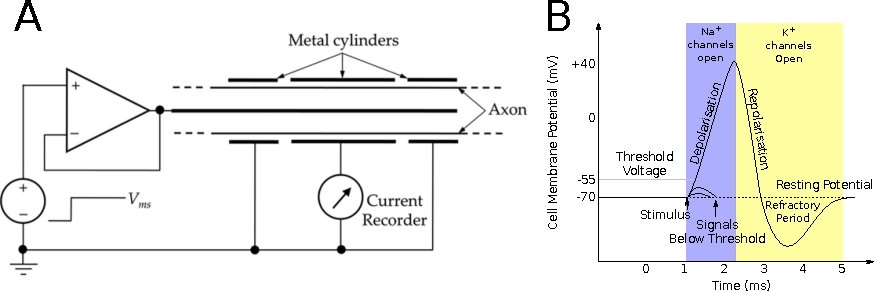
\includegraphics[width=0.9\textwidth]{figures/Hodgkin-Huxley_action_potential.pdf}
	\end{center}
	\captionsetup{singlelinecheck = false, justification=raggedright}
	\caption[The Action Potential is a Solution to the Hodkin-Huxley Model] {\textbf{The Action Potential is a Solution to the Hodgkin-Huxley Model }}{ A) The ``voltage clamp" experimental set up which was used to study nerve impulses \cite{hodgkin_huxley_figure_website}. A giant squid nerve was submerged in sea water and an electrode was threaded through it as shown. The voltage was recorded as impulses were fired into the nerve. B) The shape of the action potential is a familiar sight in many physiology textbooks. The physical basis for its shape was realised through the mathematical modelling of Hodgkin and Huxley which won them the 1963 Noble Prize in physiology or medicine. This discovery is an example of the physiological importance of ion channels and also how deep theoretical insight can lead to predictive models of living systems \cite{hodgkin1952, hodgkin1952a, hodgkin1952b, hodgkin1952c, hodgkin1952d}.}
	\label{action_potential_graphic}
\end{figure}


Equation \ref{hh_equations} is an example of the development of a mathematical formalism which is not fundamental in the same way as the equations at the beginning of section \ref{WIP} but rather, it is built for an express purpose: to model the propagation of signals through a nerve. This model shows how quantitative thinking can lead to insights in biology. The sheer complexity of biology demands this of us. We cannot create complete theories so we must find useful formalisms for small domains of the problem space.

\begin{figure}
	\begin{center}
		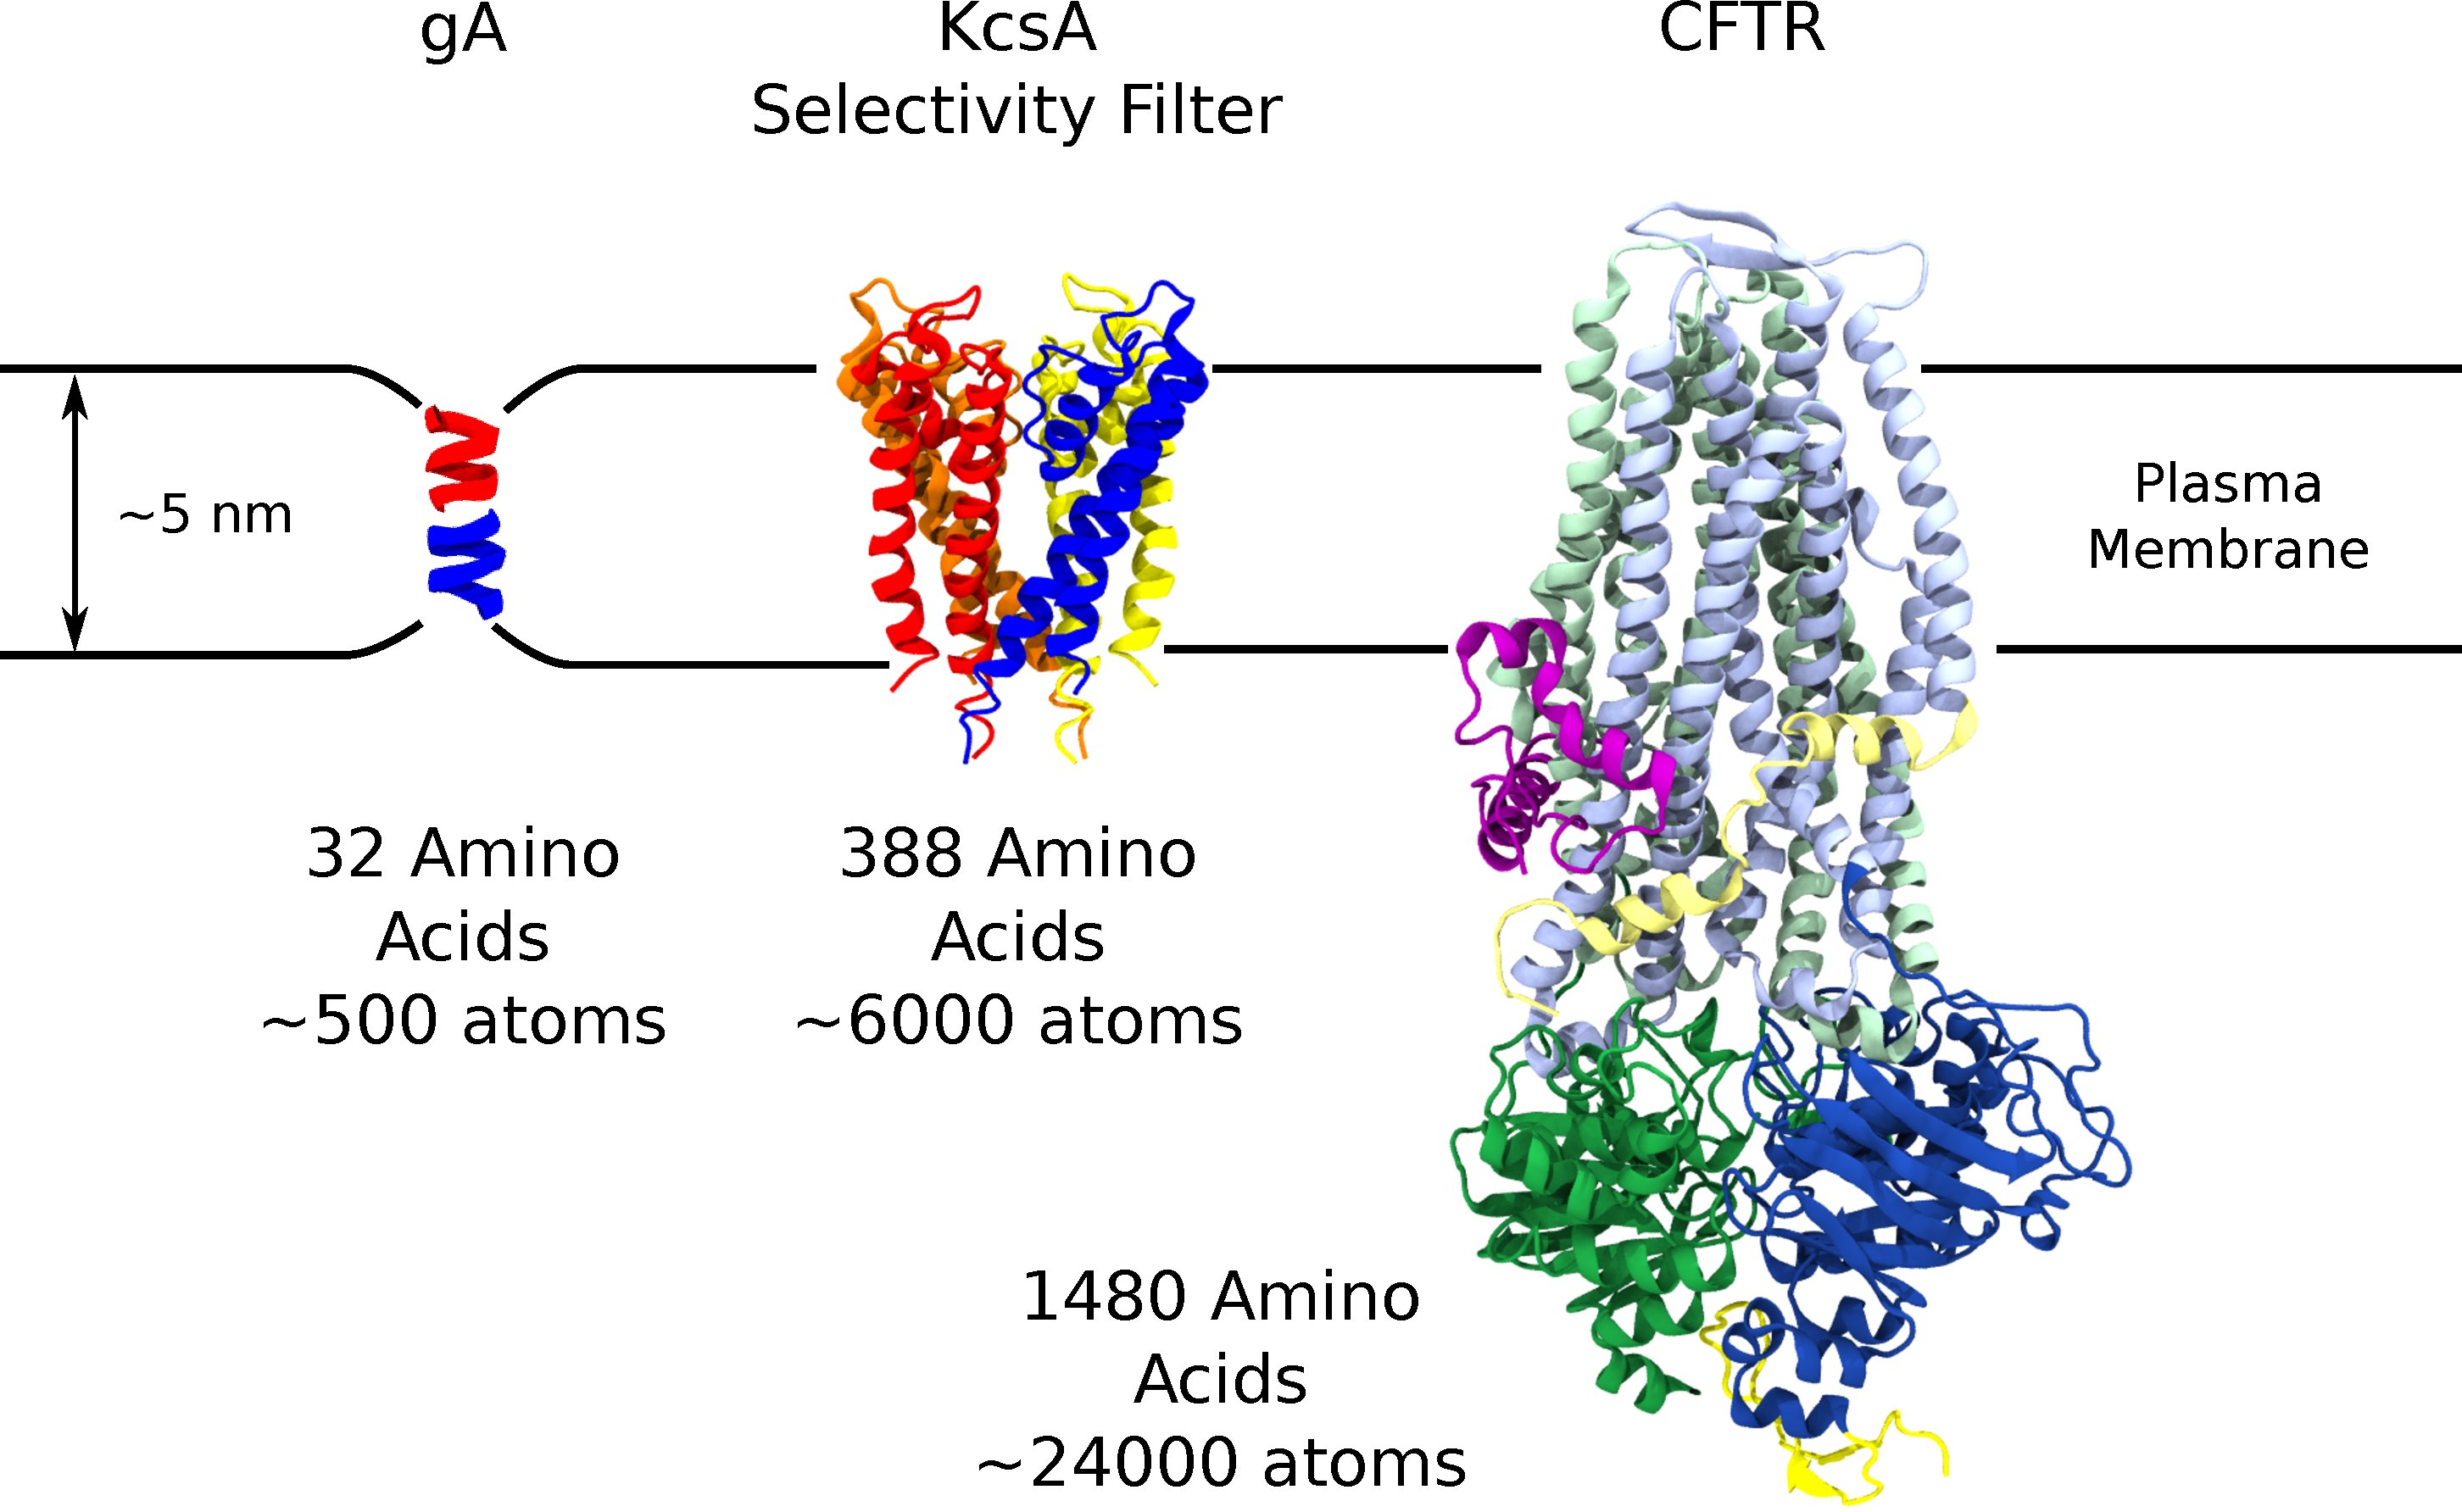
\includegraphics[width=0.8\textwidth]{figures/ion_channel_progression.pdf}
	\end{center}
	\captionsetup{singlelinecheck = false, justification=raggedright}
	\caption[Different Ion Channels Amenable to Molecular Simulation] {\textbf{Different Ion Channels Amenable to Molecular Simulation}}{Gramicidin A was initially used as a toy model to test different \textit{in silico} modelling techniques (PDB ID 1NT5) \cite{sham2003}.\footnote{Other toy systems include dialanine, deca-alanine and BPTI.} KcsA, is a bacterial potassium channel. This structure only comprises the pore domain, sometimes called the selectivity filter (PDB ID 1BL8) \cite{doyle1998}. This structure drew interest because potassium channels are play an important role in the function of cells. Finally, the CFTR anion channel which this thesis is written about (PDB ID 6MSM) \cite{zhang2018a}. In the course of 30 years that we have gone from simulating just a few nanoseconds of Gramicidin A to collecting almost half a millisecond of data in this thesis. This heralds an exciting future for computational biophysics \cite{roux1993}. What is even more exciting will be the next 30 years. At the time of writing, a computational engine named Anton 3 has come online. This purpose built computer could perform all the calculations in this thesis in less than a week \cite{jones2022, russell2021}. That's not a week in parallel, that's in serial!}
	\label{ion_channel_progress}
\end{figure}

In this thesis we aim to do something similar, by building up from the fundamental physics outlined in \ref{chap:methods} we will build a model for the disfunction of a single gene (CFTR) to understand a disease (CF). Again, we do not possess sufficient computational power to produce a complete physical model of CF, so we will have to settle for a qualitative model which we will outline in \ref{chap:conclusion}. 

%The measurements and modelling they carried out gave an exciting set of results. They found that the cell had to maintain a constant voltage gradient, they discovered that the presence of voltage gated ion channels and cation selective ion channels\cite{hodgkin1952}. Each of these features, motivated by mathematical modelling have been found to be critical to the functioning of the cell and fundamental to the foundation of molecular biophysics.    
Motivated by the advances in cell biology, that arose from the Hodgkin-Huxley model early adopters of computational biophysics such as Martin Karplus, Beno\^it Roux, Shin Ho-Chung, Mark Sanson, Serdar Kuyucak and Toby Allen also devoted significant parts of their career to studying ion channels\cite{sansom1991, roux1991, roux1993, sansom1991, allen2003, allen2004, chung2002, tieleman2001}. 

These early studies usually focussed on gramicidin A (gA) because of its small size and the availability of experimental data with which to compare theoretical. This small antibacterial peptide assembles into an ion channel in the cell walls of gram positive bacteria, bleeding them dry of potassium ions \cite{liou2015}.\footnote{Potassium is is critical to to cellular function.}

This careful work on gA aided the development of many computational techniques. Along with an abundance of protein structures and other experimental advances, of this kind of modelling and experimental techniques the molecular details of the function of ion channels has become accessible to computational techniques \cite{flood2019}. The work on gA enabled careful studies of potassium channels \cite{rashid2013, li2021, vandenberg2021}. 

Ion channels will likely continue to be important clinical targets in the future. They can be used as knobs to manipulate the behaviour of the cells they attached to. They are responsible for the sensation of pressure (and hence touch) \cite{chesler2018}, temperature \cite{castillo2018}, pain \cite{kingwell2019}, acids \cite{kweon2013}, smell (in insects) \cite{sato2008} and play a critical role in cell morphogenesis and growth \cite{lang2005, sundelacruz2009, levin2014, levin2014a}.

The availability of protein structures and the maturation of computational methods has enabled diverse studies of ion channels and other protein systems \cite{lev2020, chen2021}. This progress is summarised in figure \ref{ion_channel_progress}. In large part this explosion of interest was motivated by the careful study of ion channels. In this work we have continued this trend by applying the theoretical and computational techniques developed for studying ion channels toward developing a theoretical model of how to think about Cystic Fibrosis. 





\section{Studying Cystic Fibrosis; Toward a Molecular Theory of Disease.} 

The sad truth of Cystic Fibrosis (CF) is that those afflicted are extremely unlucky. A mutation change to their genome and their lungs fill with sticky mucus and become infected with bacteria, each breath becomes cumbersome \cite{katkin2022}. Historically, diseases have been diagnosed based on symptoms and not causes \cite{foucault1994}. As section \ref{WIP} outlines, this is antithetical to how we would like to study physical systems. To build a predictive model, we would wish to understand the root cause of a disease so we can predict how to treat it. Discovering this root cause can be extremely difficult and often requires decades of clinical enquiry \cite{dubois2016, tsui2013}. CF has the helpful characteristic of being a monogenic disease, so our molecular theory of this disease can focus on a single protein system.\footnote{Note that in a strict sense, mutations to CFTR are a necessary but not sufficient condition to developing CF. Other genetic and environmental factors are important, as with all diseases. This is simply less the case for CF.}

In this way, my motivations for studying the CFTR protein aren't solely focussed on treating disease. This problem is also an interesting opportunity to develop molecular theories of biology. 

There is a perspective on protein evolution which states that the stability of a protein's structure contributes to the overall fitness of an organisms by a formula \cite{depristo2005}:

\begin{equation}
	\label{fitness_equation}
	W(\Delta G) \propto \exp\bigg(\bigg[-\frac{\Delta G - \Delta G_{opt}}{\sigma_{\Delta G}}\bigg]^4\bigg) + c
\end{equation}

Here, $W$ represents the evolutionary fitness of an organism, $\Delta G$ is the folding energy of the protein with a given gene sequence and $\Delta G_{opt}$ is the folding energy of the protein in the average (fit) population. The parameter $\sigma_{\Delta G}$ controlls how broad this distribution will be and depends significantly on the protein physics of the gene. Figure \ref{fitness_landscape_figure} demonstrates the types of random walks of a gene through sequence space which this model predicts. 

As the $\>400$ disease causing mutations indicates\cite{cftr2}, the CFTR gene exhibits an exceptionally small $\sigma_{\Delta G}$, so the band in the modified gaussian in figure \ref{fitness_landscape_figure}a is narrow. This means that CFTR sits at the precipice of a daunting cliff in sequence space.  So by taking small steps in sequence space and figuring out what factors have caused $W$ to decrease, we can try to understand how we might push the needle of protein stability back into the optimal zone. Once we understand how we can do this for CFTR we can use such thinking to build our methods outward and apply it to other diseases, such as sickle cell anemia, Alzheimer's disease, and Huntington's disease\cite{depristo2005}.

\begin{figure}
	\begin{center}
		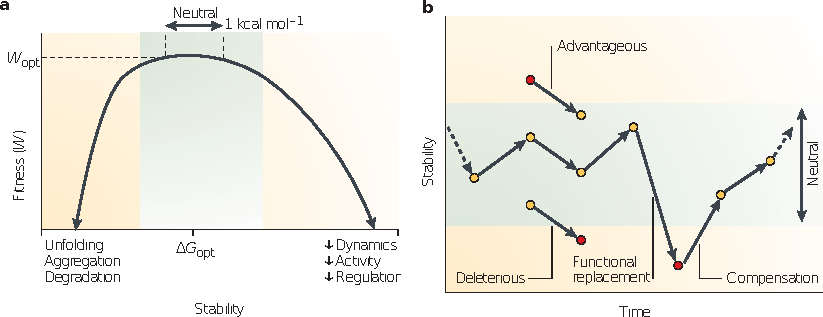
\includegraphics[width=1.0\textwidth]{figures/fitness_landscape_fig.pdf}
	\end{center}
	\captionsetup{singlelinecheck = false, justification=raggedright}
	\caption[A physical model for how to view protein evolution] {\textbf{A physical model for how to view protein evolution}}{a)The stability of a protein $\Delta G$ is related to the fitness of an organism $W$ by equation \ref{fitness_equation}. This model gives rise to a peaked distribution which helps us understand how so many mutants can give rise to cystic fibrosis. It appears as though the CFTR gene has an exceptionally narrow $\sigma_{\Delta G}$ and so small changes to the sequence of the gene have a comparatively dramatic effect on the evolutionary fitness of the organism. b) The model in equation \ref{fitness_equation} Gives rise to a random walk through in sequence space for subsequent generations. In the case of CF, it would appear as though \textit{homo sapiens} are stuck at a specific snapshot in evolutionary time where CFTR may easily lose function. So, without gene therapies which can modify a gene sequence \textit {in vivo} we must use small molecule drugs and other medical interventions to somehow broaden the peak in of equation \ref{fitness_equation}.}
	\label{fitness_landscape_figure}
\end{figure}

Due to the array of disease causing mutations which occur across the cystic fibrosis protein, there is a large body of literature on its unique function \cite{csanady2019a}. This presents the opportunity to simultaneously perform basic biophysical research while directly assisting in furthering patient outcomes. This is the sort of inquiry which drives basic science forward, combining interesting experimental data into theoretical models to make testable predictions. The aim of this thesis is to build a model to help direct efforts which will produce better patient outcomes. In chapter \ref{chap:conclusion} we will combine evidence from the existing literature as well as our biochemical and simulation results in order to build our predictive model for which outlines future strategies to treat CF.

As we will see in chapter \ref{chap:cftr} the integration of basic biological research into the treatment of disease can drastically improve patient outcomes. In this particular context, we have studied a single gene. But eventually, similar thinking will be able to build out our understanding consider multiple genes in as much detail, giving us a more complete picture of both life and disease, heralding the exciting future for biophysics. 

\section{The Future is Biological}
Biology has particularly important applications in medicine, agriculture and increasingly, manufacturing \cite{anonymous2019, scown2022}. We are on the cusp of developing it from a descriptive to a predictive science \cite{kochanski1973,liu2005, mogilner2016, covert2021, jumper2021}. This transition is being driven by the combination of advanced of experimental techniques, rich datasets, strong theories and powerful computational engines. This is particularly exciting as biological systems have happened upon ingenious problems to some very difficult problems through evolution \cite{dawkins1989}. It has much of the hard work for us, and as we understand it better we can begin to apply its logic to our own problems \cite{benyus2009}.

Throughout science, the integration of experimental data with theoretical models leads to new discoveries. In the case of biology, wet lab scientists take advantage of experimental techniques which allow them to understand the structure and dynamics of living things from the top down. The finer the experimental instrument, the finer the detail they may resolve. Conversely, computational and theoretical biologists take a bottom up approach. We aim to take the granular details of a system, and integrate them upwards to model the macroscopic behaviour of that system. 

With more powerful computers and more detailed theoretical models, we can make predictions about the behaviour of more complex systems. What is so exciting about the current era of biological research is that the domains of these two approaches are beginning to overlap, where they can synergize  and drive further breakthroughs\cite{anonymous2019}.

This has been happening in physics for decades. Resulting in world changing breakthroughs like telecommunications, nuclear power and transistors \cite{wu2009}. The reason this has been possible for physicists is that the systems they usually study study are homogeneous. They include just a few, albeit sometimes complex components. Hence, it is much easier to integrate a theoretical formalism upward to predict measurable phenomenon. 

The difference with biological systems is that they have so many different components. Hence, finding an analytic or even computationally tractable solution is usually impossible. However, as we collect more data with experimental techniques\footnote{Important biophysical techniques which one will encounter often in the literature are cryogenic electron microscopy (Cryo-EM) \cite{cheng2015, callaway2015, callaway2020}, electrophysiology \cite{aidley1996}, nuclear magnetic resonance (NMR) spectroscopy \cite{marion2013}, confocal and fluorescence microscopy \cite{sanderson2014}, X-ray Crystallography \cite{frauenfelder2010, drenth2006}, and genetic engineering (explanations of CRISPR-Cas9 or inverse PCR based techniques can be found in \cite{silva2017} and \cite{crispr2019} respectively)} and build more powerful computers we can approach more complete models. These in turn inform more powerful theoretical models which help direct the material efforts of experimental studies. 

Now that an overview of the philosophy behind physical biology, how we intend to apply it to study CF, and the exciting future which will this philosophy will soon usher in, we will dive deep into atomistic theoretical models which we will use to study the CFTR protein. 

%Armed with this philosophy we will delineate how to use the formal object of the Schr\"oedinger wave equation to make approximations to atomic systems in order to create a biophysical model for macromolecular systems like proteins.
